%!QXV0b3I6IFRvbSBTdPZocmVy

\documentclass[11pt, paper=A4]{scrartcl} % Dokumentenklasse: Artikel im KOMA-Script-Format, 11pt Schriftgröße, A4 Papierformat

\usepackage[utf8]{inputenc} % Ermöglicht die Eingabe von UTF-8 Zeichen
\usepackage[ngerman]{babel} % Deutsche Sprachunterstützung (z.B. für Silbentrennung und Datum)
\usepackage{marvosym} % Symbole wie Eurozeichen und andere spezielle Symbole
\usepackage{gensymb,siunitx} % Einheiten und mathematische Symbole, siunitx für konsistente Darstellung von Einheiten
\usepackage{amsmath} % Erweiterte mathematische Umgebungen und Symbole
\usepackage{amssymb} % Zusätzliche mathematische Symbole
\usepackage{pgfplots, relsize} % Erstellung von Plots und Diagrammen, relsize für relative Schriftgrößenanpassung
\usepackage{circuitikz} % Zeichnen von elektrischen Schaltkreisen
\usepackage{xcolor} % Farbunterstützung
\usepackage{cancel} % Durchstreichen von mathematischen Ausdrücken
\usepackage{icomma} % Intelligente Kommas in mathematischen Ausdrücken
\usepackage{endnotes} % Endnoten anstelle von Fußnoten
\usepackage{graphicx} % Einfügen und Anpassen von Grafiken
\usepackage{longtable} % Tabellen, die über mehrere Seiten gehen können
\usepackage{booktabs} % Professionelle Tabellen mit \toprule, \midrule und \bottomrule
\usepackage[automark,headsepline,footsepline]{scrlayer-scrpage} % Anpassung von Kopf- und Fußzeilen
\usepackage{geometry} % Anpassung der Seitenränder und des Seitenlayouts
\usepackage[default,oldstyle,scale=0.95]{opensans} % Schriftart Open Sans
\usepackage{lmodern} % Latin Modern Schriftart
\usepackage[T1]{fontenc} % T1 Schriftkodierung für bessere Trennung und Darstellung
\usepackage[]{hyperref} % Erzeugt Hyperlinks im Dokument ([hidelinks] entfernt farbige Markierung)
\usepackage{enumitem} % Anpassung der Aufzählungszeichen und Listen
\usepackage{subfig} % Einfügen von Unterabbildungen innerhalb einer Abbildung
\usepackage{caption} % Anpassung der Beschriftungen von Abbildungen und Tabellen
\usepackage{float} % Bessere Kontrolle über die Platzierung von Gleitobjekten (z.B. Tabellen, Abbildungen)

%%%%%%%%%%%%%%%%%%%%%%%%%%%%%%%%%%%%%%%%%%%%%%%%%%%%%%%%%%%%%%%%%%%%%%%%%%%%%%%
%%%%%%%%%%%%%%%%%%%%%%%%%%%%%%%%%%%%%%%%%%%%%%%%%%%%%%%%%%%%%%%%%%%%%%%%%%%%%%%
%%%%%%%%%%%%%%%%%%%%%%%%%%%%%%%%%%%%%%%%%%%%%%%%%%%%%%%%%%%%%%%%%%%%%%%%%%%%%%%
% Seitenabstände

\geometry{
  a4paper,
  left=1.9cm,
  right=1.9cm,
  top=2.5cm,
  bottom=3.1cm,
}

%%%%%%%%%%%%%%%%%%%%%%%%%%%%%%%%%%%%%%%%%%%%%%%%%%%%%%%%%%%%%%%%%%%%%%%%%%%%%%%
%%%%%%%%%%%%%%%%%%%%%%%%%%%%%%%%%%%%%%%%%%%%%%%%%%%%%%%%%%%%%%%%%%%%%%%%%%%%%%%
%%%%%%%%%%%%%%%%%%%%%%%%%%%%%%%%%%%%%%%%%%%%%%%%%%%%%%%%%%%%%%%%%%%%%%%%%%%%%%%
% Variablen

\title{ETP1} % Titel des Dokuments

% Definiert das Thema, das auf dem Deckblatt und in der Kopfzeile verwendet wird
\newcommand{\thema}{Beispielthema}

% Definiert den ersten Autor und seine Matrikelnummer
\newcommand{\autorEins}{John Hallo} % ist Protokollführer
\newcommand{\autorEinsMnr}{4242420}

% Definiert den zweiten Autor und seine Matrikelnummer
\newcommand{\autorZwei}{Max Mustermann}
\newcommand{\autorZweiMnr}{1234567}

% Definiert den dritten Autor und seine Matrikelnummer
\newcommand{\autorDrei}{David Meier}
\newcommand{\autorDreiMnr}{7654321}

% Definiert die Gruppennummer
\newcommand{\gruppe}{2}

% Setzt die Autoren des Dokuments
\author{\autorEins\space und \autorZwei}

% Erklärung:
% Diese Variablen werden im gesamten Dokument verwendet, um konsistent Informationen wie Titel, Thema, Autoren und Gruppennummer anzuzeigen.
% Änderungen an diesen Variablen werden automatisch an allen Stellen im Dokument übernommen, wo sie referenziert werden.

%%%%%%%%%%%%%%%%%%%%%%%%%%%%%%%%%%%%%%%%%%%%%%%%%%%%%%%%%%%%%%%%%%%%%%%%%%%%%%%
%%%%%%%%%%%%%%%%%%%%%%%%%%%%%%%%%%%%%%%%%%%%%%%%%%%%%%%%%%%%%%%%%%%%%%%%%%%%%%%
%%%%%%%%%%%%%%%%%%%%%%%%%%%%%%%%%%%%%%%%%%%%%%%%%%%%%%%%%%%%%%%%%%%%%%%%%%%%%%%
% Farben, Schriftarten und Abstände

% Farben definieren
\definecolor{hauptblau}{cmyk}{1, 0.7, 0, 0.06} % Hauptblau
\definecolor{hellblau}{cmyk}{0.42, 0.16, 0.04, 0} % Hellblau
\definecolor{mittelblau}{cmyk}{0.85, 0.21, 0, 0} % Mittelblau

% Standardschriftart auf serifenlose Schrift setzen
\renewcommand{\familydefault}{\sfdefault}

% Schriftart für Abschnittsüberschriften ändern
\addtokomafont{sectioning}{\usefont{T1}{lmr}{m}{n}\sffamily\bfseries}

% Abschnittsnummerierung deaktivieren
\setcounter{secnumdepth}{0}

% Einrückung der ersten Zeile eines Absatzes deaktivieren
\setlength{\parindent}{0pt}

% Abstand vor und nach Abschnittsüberschriften ändern
\RedeclareSectionCommands[
  beforeskip=1\baselineskip, % Abstand vor der Überschrift
  afterskip=0.5\baselineskip % Abstand nach der Überschrift
]{section,subsection,subsubsection}

% Farbe der Abschnittsüberschriften auf Hauptblau setzen
\addtokomafont{section}{\color{hauptblau}}
\addtokomafont{subsection}{\color{hauptblau}}


%%%%%%%%%%%%%%%%%%%%%%%%%%%%%%%%%%%%%%%%%%%%%%%%%%%%%%%%%%%%%%%%%%%%%%%%%%%%%%%
%%%%%%%%%%%%%%%%%%%%%%%%%%%%%%%%%%%%%%%%%%%%%%%%%%%%%%%%%%%%%%%%%%%%%%%%%%%%%%%
%%%%%%%%%%%%%%%%%%%%%%%%%%%%%%%%%%%%%%%%%%%%%%%%%%%%%%%%%%%%%%%%%%%%%%%%%%%%%%%
% Graphiken und Bilder

% Benenne die automatisch generierte Bildunterschrift um
\renewcommand*\figurename{Abbildung}

% Definiere \includegraphics neu, um eine maximale Breite festzulegen, wenn das Bild größer als \linewidth ist
\let\oldincludegraphics\includegraphics
\renewcommand{\includegraphics}[2][]{%
  \begin{center}
    \oldincludegraphics[width=0.8\linewidth,keepaspectratio]{#2}%
  \end{center}
}

% Erstelle einen benutzerdefinierten Befehl für Kopfzeilenbilder
\newcommand{\headerimage}[2][]{\oldincludegraphics[#1]{#2}}

% Definiere die figure-Umgebung neu, um die Reihenfolge nie zu ändern
\let\oldfigure\figure
\let\endoldfigure\endfigure
\renewenvironment{figure}[1][H]{\oldfigure[#1]}{\endoldfigure}


%%%%%%%%%%%%%%%%%%%%%%%%%%%%%%%%%%%%%%%%%%%%%%%%%%%%%%%%%%%%%%%%%%%%%%%%%%%%%%%
%%%%%%%%%%%%%%%%%%%%%%%%%%%%%%%%%%%%%%%%%%%%%%%%%%%%%%%%%%%%%%%%%%%%%%%%%%%%%%%
%%%%%%%%%%%%%%%%%%%%%%%%%%%%%%%%%%%%%%%%%%%%%%%%%%%%%%%%%%%%%%%%%%%%%%%%%%%%%%%
% Quellen

% Benenne die automatisch generierte Quellenüberschrift um
\renewcommand{\notesname}{Quellen und Anmerkungen}

%%%%%%%%%%%%%%%%%%%%%%%%%%%%%%%%%%%%%%%%%%%%%%%%%%%%%%%%%%%%%%%%%%%%%%%%%%%%%%%
%%%%%%%%%%%%%%%%%%%%%%%%%%%%%%%%%%%%%%%%%%%%%%%%%%%%%%%%%%%%%%%%%%%%%%%%%%%%%%%
%%%%%%%%%%%%%%%%%%%%%%%%%%%%%%%%%%%%%%%%%%%%%%%%%%%%%%%%%%%%%%%%%%%%%%%%%%%%%%%
% Kopf- und Fußzeilen

\clearpairofpagestyles % Löscht alle voreingestellten Seitenstile

% Kopfzeile innen: Bild linksbündig
\ihead{\raisebox{-0.7\baselineskip}{\headerimage[height=1.2cm,keepaspectratio]{./assets/HAW.jpg}}}

\chead{} % Kopfzeile zentriert: leer

% Kopfzeile außen: Thema rechtsbündig
\ohead{\textcolor{hauptblau}{\raisebox{-0.8\baselineskip}{\thema}}}

% Fußzeile innen: Autoreninformationen linksbündig
\ifoot{\textcolor{hauptblau}{\raisebox{-0.3\baselineskip}{\autorEins , \autorZwei\space und \autorDrei}}}

\cfoot{} % Fußzeile zentriert: leer

% Fußzeile außen: Seitenzahl rechtsbündig
\ofoot{\textcolor{hauptblau}{\raisebox{-0.3\baselineskip}{\thepage}}}

% Optionen für Kopf- und Fußzeilenlinien
\KOMAoptions{headsepline=.5pt, footsepline=.5pt}

% Farbe der Kopfzeilenlinie setzen
\addtokomafont{headsepline}{\color{hauptblau}}

% Farbe der Fußzeilenlinie setzen
\addtokomafont{footsepline}{\color{hauptblau}}

% Schriftart für Kopf- und Fußzeilen setzen
\addtokomafont{pageheadfoot}{\normalfont}

%%%%%%%%%%%%%%%%%%%%%%%%%%%%%%%%%%%%%%%%%%%%%%%%%%%%%%%%%%%%%%%%%%%%%%%%%%%%%%%
%%%%%%%%%%%%%%%%%%%%%%%%%%%%%%%%%%%%%%%%%%%%%%%%%%%%%%%%%%%%%%%%%%%%%%%%%%%%%%%
%%%%%%%%%%%%%%%%%%%%%%%%%%%%%%%%%%%%%%%%%%%%%%%%%%%%%%%%%%%%%%%%%%%%%%%%%%%%%%%
% Titelseite

% Beginn des Dokuments
\begin{document}

% Beginn der Titelseite
\begin{titlepage}
  \makeatletter

    % Kopfzeilenbild linksbündig
    \begin{flushleft}
      \headerimage[width=0.4\textwidth]{./assets/HAW.jpg} % Bild der HAW linksbündig
    \end{flushleft}
    \vspace{3.6cm} % Abstand nach unten

    % Titel und Thema zentriert
    \begin{center}
      \fontsize{50}{60}\selectfont \textbf{\textcolor{hauptblau}{\@title}}\\ % Titel in 50pt, dick und blau
      \vspace{-1cm} % Abstand nach oben verkleinern
      {\LARGE \textbf{\textcolor{hellblau}{\thema}}}\par
    \end{center}
    
    % Gruppen- und Autoreninformationen am unteren Rand der Seite
    \vfill

    \begin{flushright}
      \begin{minipage}{0.4\textwidth}
        {\large \textbf{Gruppe: \gruppe}}\par
        \vspace{0.5cm} % Abstand nach unten

        \raggedright 

        \setlength{\baselineskip}{1.5em} % Zeilenabstand einheitlich setzen
        {\large \textsf{\autorEins\\Matrikel-Nr.: \autorEinsMnr\\(Protokollführer)}}\par

        \vspace{0.5cm} % Abstand nach unten

        {\large \textsf{\autorZwei\\Matrikel-Nr.: \autorZweiMnr}}\par

        \vspace{0.5cm} % Abstand nach unten
          
        {\large \textsf{\autorDrei\\Matrikel-Nr.: \autorDreiMnr}}\par
      \end{minipage}
    \end{flushright}

  \makeatother
\end{titlepage}

%%%%%%%%%%%%%%%%%%%%%%%%%%%%%%%%%%%%%%%%%%%%%%%%%%%%%%%%%%%%%%%%%%%%%%%%%%%%%%%
%%%%%%%%%%%%%%%%%%%%%%%%%%%%%%%%%%%%%%%%%%%%%%%%%%%%%%%%%%%%%%%%%%%%%%%%%%%%%%%
%%%%%%%%%%%%%%%%%%%%%%%%%%%%%%%%%%%%%%%%%%%%%%%%%%%%%%%%%%%%%%%%%%%%%%%%%%%%%%%
% Inhalt

\tableofcontents

\thispagestyle{empty}

\newpage

\setcounter{page}{1}

%%%%%%%%%%%%%%%%%%%%%%%%%%%%%%%%%%%%%%%%%%%%%%%%%%%%%%%%%%%%%%%%%%%%%%%%%%%%%%%

\section{Tabellen}\label{tabellen}

\begin{table}[H] % Tabelle mit fester Positionierung
  \centering
  \begin{tabular}{|l|c|r|} % Tabelle mit drei Spalten: linksbündig, zentriert, rechtsbündig
    \hline
    \textbf{Spalte 1} & \textbf{Spalte 2} & \textbf{Spalte 3} \\ % Kopfzeile
    \hline
    Eintrag 1 & Eintrag 2 & Eintrag 3 \\ % Erste Zeile
    \hline
    Eintrag 4 & Eintrag 5 & Eintrag 6 \\ % Zweite Zeile
    \hline
    Eintrag 7 & Eintrag 8 & Eintrag 9 \\ % Dritte Zeile
    \hline
  \end{tabular}
  \caption{Beispieltabelle} % Tabellenunterschrift
  \label{tab:example} % Label für Referenzierung
\end{table}

Siehe Tabelle \ref{tab:example} % Referenz auf die Tabelle

%%%%%%%%%%%%%%%%%%%%%%%%%%%%%%%%%%%%%%%%%%%%%%%%%%%%%%%%%%%%%%%%%%%%%%%%%%%%%%%

\section{Mathe}\label{mathe}

\[
\begin{aligned}
  \int_{0}^{\infty} e^{-x^2} \cos(\pi x) \, dx = \frac{\sqrt{\pi}}{2} e^{-\pi^2/4}
\end{aligned}
\]

%%%%%%%%%%%%%%%%%%%%%%%%%%%%%%%%%%%%%%%%%%%%%%%%%%%%%%%%%%%%%%%%%%%%%%%%%%%%%%%

\section{Grafiken}\label{grafiken}

\subsection{Funktionen}\label{funktionen}

\begin{figure}[H]\centering % Zentrierte Figur mit fester Position

  \begin{tikzpicture}
    \definecolor{col1}{cmyk}{1, 0.7, 0, 0.06} % Hauptblau
    \definecolor{col2}{cmyk}{0.42, 0.16, 0.04, 0} % Hellblau
    \definecolor{col3}{cmyk}{0.85, 0.21, 0, 0} % Mittelblau

    \begin{axis}[
      samples=300, % Anzahl der Abtastpunkte
      xmax=8.5, xmin=-8, ymax=4.5, ymin=-4, % Achsengrenzen
      axis lines=left, % Achsenlinien links
      y=0.75cm, x=0.75cm, % Skalierung der Achsen
      grid=both, % Gitterlinien
      xtick={-100,...,100}, ytick={-100,...,100}, % Achsenbeschriftung
      compat=newest,
      xlabel=$x$, xlabel style={at={(1,0)}, anchor=west}, % x-Achsenbeschriftung
      ylabel=$y$, ylabel style={rotate=-90,at={(0,1)}, anchor=south}, % y-Achsenbeschriftung
      every axis plot/.append style={thick} % Linienstil
    ]
      \draw (-50,0) -- (50,0); % x-Achse
      \draw (0,-50) -- (0,50); % y-Achse

      \addplot[col1, domain=-10:10]{4*sin(3*deg(x))}; % Sinuskurve
      \addlegendentry{$f(x)=4\sin(3x)$} % Legende

      \draw[fill] (1,1) circle [radius=2pt]; % Punkt bei (1,1)
      \node[above right] at (1,1) {Punkt}; % Beschriftung des Punktes
      
    \end{axis}
  \end{tikzpicture}

\caption{Sinus Kurve}\label{fig:graph} % Beschriftung und Label
\end{figure}

%%%%%%%%%%%%%%%%%%%%%%%%%%%%%%%%%%%%%%%%%%%%%%%%%%%%%%%%%%%%%%%%%%%%%%%%%%%%%%%

\subsection{Schaltkreise}\label{schaltkreise}

\begin{figure}[H]\centering % Zentrierte Figur mit fester Position

  \begin{circuitikz}[european,] % Europäische Schaltsymbole
    \draw
    (0,0) to[voltage source, v<=$U_q$, a=$10V$] (0,3) % Spannungsquelle
          to[R, l=$R_1$, a=$1\Omega$,i=$I_1$] (3,3) % Widerstand R1
          to[R, l=$R_3$, a=$21\Omega$, i=$I_3$] (6,3) % Widerstand R3
          to[R, l=$R_4$, a=$20\Omega$] (6,0) % Widerstand R4
          -- (3,0)
          -- (0,0);
    \draw
    (3,3) to[short, *-, i>_=$I_2$] (3,2) % Verbindung mit Strom I2
          to[R, l=$R_2$, a=$9\Omega$] (3,1) % Widerstand R2
          to[short, -*] (3,0)
    ;
    \node at (1.5,1.5) {$1$}; % Knoten 1
    \node at (4.5,1.5) {$2$}; % Knoten 2
  \end{circuitikz}

\caption{Schaltkreis}\label{fig:cir} % Beschriftung und Label
\end{figure}

%%%%%%%%%%%%%%%%%%%%%%%%%%%%%%%%%%%%%%%%%%%%%%%%%%%%%%%%%%%%%%%%%%%%%%%%%%%%%%%

\subsection{Bilder}\label{bilder}

\begin{figure}
\centering
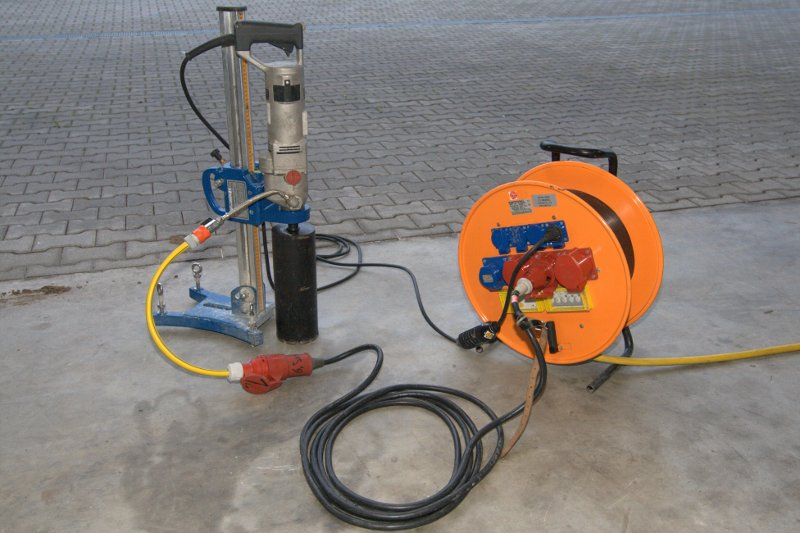
\includegraphics[keepaspectratio]{./assets/image.png}
\caption{Bild von \href{https://www.thw-viernheim.de/berichte/archiv/2011/neuer-adapter-ermoeglicht-wasserversorgung-ueber-aggregate.html}{THW Ortsverband Viernheim}}\label{fig:id}
\end{figure}

%%%%%%%%%%%%%%%%%%%%%%%%%%%%%%%%%%%%%%%%%%%%%%%%%%%%%%%%%%%%%%%%%%%%%%%%%%%%%%%

\section{Formatierung}\label{formatierung} % Abschnitt für Formatierung

\subsection{Text}\label{text} % Unterabschnitt für Text

\subsubsection{Links}\label{links} % Unterunterabschnitt für Links

% Beispiel für einen Link zu einer Website
Es folgt ein Link zu einer \href{https://pandoc.org/}{Website}

\subsubsection{Verlinkungen zu Graphiken}\label{verlinkungen-zu-graphiken} % Unterunterabschnitt für Verlinkungen zu Graphiken

% Beispiel für Verlinkungen zu Abbildungen
Siehe wichtiges Bild Abb.~\ref{fig:id}

Siehe Schaltkreis Abb.~\ref{fig:cir}

Siehe Graphen Abb.~\ref{fig:graph}

\subsubsection{Quellen}\label{quellen} % Unterunterabschnitt für Quellen

% Beispiel für eine Quelle in den Endnoten
Diese Information stammt aus einer wichtigen Quelle.\endnote{Link zur \href{https://quelle.com}{Quelle}}

\subsubsection{Fließtext}\label{fließtext} % Unterunterabschnitt für Fließtext

% Beispiel für Fließtext
Dies ist ein Beispiel für Fließtext. Hier können Sie normalen Text schreiben, der in Absätzen formatiert ist.


\sum \neq 

\subsubsection{Aufzählung}\label{aufzählung} % Unterunterabschnitt für Aufzählung

% Beispiel für eine Aufzählung
\begin{itemize}
  \item Erster Punkt
  \item Zweiter Punkt
  \item Dritter Punkt
\end{itemize}

\newpage

\AtEndDocument{\theendnotes}

\end{document}